%% ****** Start of file apstemplate.tex ****** %
%%
%%
%%   This file is part of the APS files in the REVTeX 4 distribution.
%%   Version 4.1r of REVTeX, August 2010
%%
%%
%%   Copyright (c) 2001, 2009, 2010 The American Physical Society.
%%
%%   See the REVTeX 4 README file for restrictions and more information.
%%
%
% This is a template for producing manuscripts for use with REVTEX 4.0
% Copy this file to another name and then work on that file.
% That way, you always have this original template file to use.
%
% Group addresses by affiliation; use superscriptaddress for long
% author lists, or if there are many overlapping affiliations.
% For Phys. Rev. appearance, change preprint to twocolumn.
% Choose pra, prb, prc, prd, pre, prl, prstab, prstper, or rmp for journal
%  Add 'draft' option to mark overfull boxes with black boxes
%  Add 'showpacs' option to make PACS codes appear
%  Add 'showkeys' option to make keywords appear
%\documentclass[aps,prl,preprint,groupedaddress]{revtex4-1}
%\documentclass[aps,prl,preprint,superscriptaddress,showpacs]{revtex4-1}
%\documentclass[aps,pre,preprint,superscriptaddress,showpacs]{revtex4-1}
%\documentclass[aps,prl,reprint,groupedaddress]{revtex4-1}
\documentclass[aps,prl,preprint,superscriptaddress,showkeys,linenumbers]{revtex4-1}

% You should use BibTeX and apsrev.bst for references
% Choosing a journal automatically selects the correct APS
% BibTeX style file (bst file), so only uncomment the line
% below if necessary.
%\bibliographystyle{apsrev4-1}

%%% Packages
\usepackage{upgreek} %%% This enables non-italic greek letters.
\usepackage{amsmath}
\usepackage{graphicx}
\usepackage{ctable}
%\setcitestyle{authoryear,round}%Setting citation style. Changing braces to ()
\setcitestyle{open={},close={},authoryear,semicolon}%Setting citation style no parenthesis between the year.

%\usepackage{lineno} %line numbers
%%% Tracked Revision

\definecolor{Antonio}{rgb}{1,0,0}

\begin{document}

% Tracked Revision 



% Use the \preprint command to place your local institutional report
% number in the upper righthand corner of the title page in preprint mode.
% Multiple \preprint commands are allowed.
% Use the 'preprintnumbers' class option to override journal defaults
% to display numbers if necessary
%\preprint{}

%Title of paper
%\title{Unifying framework for the diffusion of microscopic particles in mucus}
%\title{\textcolor{Antonio}{Emerging properties obtained from the meta-analysis of particle diffusion in mucus}}
%\title{\textcolor{Antonio}{Theoretical framework of particle diffusion in mucus based on empirical meta-analysis}}
%\title{\textcolor{Antonio}{Empirical meta-analysis and theoretical framework of microscopic particles diffusion in mucus}}
%\title{\textcolor{Antonio}{Empirical and theoretical meta-analysis of microscopic particles diffusion in mucus}}
\title{Empirical and theoretical analysis of particle diffusion in mucus}

\author{Antonio Cobarrubia}
\email{tony.cobarrubia38@gmail.com}
\author{Jarod Tall}
\email{jarod.tall@gmail.com}
\author{Austin Crispin-Smith}
\email{augustuscrispin@gmail.com}
\affiliation{Viral Information Institute, San Diego State University, San Diego, CA 92182, USA}%Lines break automatically or can be forced with \\
\affiliation{Department of Physics, San Diego State University, San Diego, CA 92182, USA}
\author{Antoni Luque} 
\email{aluque@sdsu.edu}
\affiliation{Viral Information Institute, San Diego State University, San Diego, CA 92182, USA}
\affiliation{Department of Mathematics and Statistics, San Diego State University, San Diego, CA 92182, USA}
\affiliation{Computational Science Research Center, San Diego State University, San Diego, CA 92182, USA}
% \email{Second.Author@institution.edu}
%\affiliation{%
% Authors' institution and/or address\\
% This line break forced with \textbackslash\textbackslash
%}%

% repeat the \author .. \affiliation  etc. as needed
% \email, \thanks, \homepage, \altaffiliation all apply to the current
% author. Explanatory text should go in the []'s, actual e-mail
% address or url should go in the {}'s for \email and \homepage.
% Please use the appropriate macro foreach each type of information

% \affiliation command applies to all authors since the last
% \affiliation command. The \affiliation command should follow the
% other information
% \affiliation can be followed by \email, \homepage, \thanks as well.
%\author{}
%\email[]{Your e-mail address}
%\homepage[]{Your web page}
%\thanks{}
%\altaffiliation{}
%\affiliation{}

%Collaboration name if desired (requires use of superscriptaddress
%option in \documentclass). \noaffiliation is required (may also be
%used with the \author command).
%\collaboration can be followed by \email, \homepage, \thanks as well.
%\collaboration{}
%\noaffiliation

\date{\today}

\begin{abstract}
Mucus is a complex fluid that coats multiple organs in animals. Various physicochemical properties can alter the diffusion of microscopic particles in mucus, impacting drug delivery, virus infection, and disease development. The simultaneous effect of these physicochemical properties in particle diffusion, however, remains elusive. Here, we analyzed 106 published experiments to identify the most dominant factors controlling particle diffusion in mucus. The effective diffusion---defined using a one-second sampling time window across experiments---spanned seven orders of magnitude, from $10^{-5}$ to $10^2$ $\upmu$m$^2$/s. Univariate and multivariate statistical analyses identified the anomalous exponent (\textcolor{Antonio}{the logarithmic slope of the mean-squared displacement}) as the strongest predictor of the effective diffusion, revealing an exponential relationship that explained 89$\%$ of the variance. A theoretical scaling analysis \textcolor{Antonio}{revealed that the stronger correlation of the anomalous exponent over the generalized diffusion constant occurs for sampling times} two orders of magnitude larger than the characteristic molecular (or local) displacement time.
\textcolor{Antonio}{This result predicts that, at these time scales, the molecular properties controlling the anomalous exponent, like particle-mucus unbinding times or particle-to-mesh size ratio---which depend on the underlying subdiffusion's mechanism---would be the most relevant physicochemical factors involved in the passive microrheology of particles in mucus.}
Our findings contrast with the fact that only one-third of the studies measured the anomalous exponent, \textcolor{Antonio}{and most experiments did not report the associated molecular properties predicted to dominate the motion of particles in mucus.}
\textcolor{Antonio}{The theoretical foundation of our work can be extrapolated to other systems, providing a guide to identify dominant molecular mechanisms regulating the mobility of particles in mucus and other polymeric fluids.}
\end{abstract}

% insert suggested PACS numbers in braces on next line
%\pacs{66.10.Cb} % Nonelectronic transport properties of condensed matter: Diffusion and thermal diffusion
% insert suggested keywords - APS authors don't need to do this
\keywords{mucus, microscopic particles, meta-analysis, random forest, subdiffusion, scaling analysis.}

%\maketitle must follow title, authors, abstract, \pacs, and \keywords
\maketitle

% body of paper here - Use proper section commands
% References should be done using the \cite, \ref, and \label commands
%\section{}
% Put \label in argument of \section for cross-referencing
%\section{\label{}}
%\subsection{}
%\subsubsection{}

% If in two-column mode, this environment will change to single-column
% format so that long equations can be displayed. Use
% sparingly.
%\begin{widetext}
% put long equation here
%\end{widetext}
%\begin{linenumbers}
\section*{Introduction}

Mucus is a complex fluid secreted by animals (\cite{SpagnSPRINGER2015,Krajina2017ACS}). It protects organs against the invasion of pathogens and promotes the interaction with commensal microbes (\cite{Backhed2005,Bakshani2018,Silveira2016}). 
\textcolor{Antonio}{The diffusivity of particles in mucus is paramount for animal health. The infectivity of animal viruses, like HIV, decreases when their diffusion in mucus is impeded (\cite{LaiJVirol2009}). On the flip side, enhancing the diffusivity of biomolecules in mucus facilitates the delivery of medical drugs in the body (\cite{ConeAdvDDM2009}), and reducing the diffusivity of commensal viruses that infect bacteria in the gut can increase their infectivity and protection against pathogens (\cite{BarrPNAS2013, BarrPNAS2015}). Multiple factors modify the diffusivity of particles in mucus, including particle size (\cite{Amsden1999, ConeAdvDDM2009}), particle charge and ionic strength (\cite{AbdulEurPharBioJ2015, ArendsLangmuir2013, HansingEurPHYSJ2016, LeilegBiophyscial2010, LIBiophysical2013}), pH (\cite{CelliPNAS2009, LaiJVirol2009, LeilegBiophyscial2010, SpagnSPRINGER2015, SukNanomedicine2011}), and the concentration and polymeric organization of the characteristic glycoproteins in mucus called mucins (\cite{BarrPNAS2015}). However, the combined effect of these physicochemical factors controlling particle diffusion in mucus remains puzzling.}

\textcolor{Antonio}{Small biomolecules and biomolecular complexes tend to diffuse more readily through mucus, while larger particles are caught in the mucin network (\cite{Amsden1999, ConeAdvDDM2009}). On the other hand, non-adhesive polystyrene particles with a diameter of 500 nm diffuse faster than smaller particles (200 nm) of the same type (\cite{LaiPNAS2007}). These contrasting results highlight the major impact of parameters other than size in particle diffusion in mucus. In fact, neutrally charged particles display higher diffusivity in mucus than charged particles of the same size with a net negative charge (\cite{AbdulEurPharBioJ2015, ArendsLangmuir2013, HansingEurPHYSJ2016, LeilegBiophyscial2010, LIBiophysical2013}). An increase in salt concentration shields charged particles, leading to diffusivities similar to neutrally charged particles (\cite{ArendsLangmuir2013, LeilegBiophyscial2010, HansingEurPHYSJ2016}). Low pH increases the distribution of negative charges in mucins and alters mucus' viscoelasticity, reducing the diffusivity of most particles (\cite{CelliPNAS2009, LaiJVirol2009, LeilegBiophyscial2010, SpagnSPRINGER2015, SukNanomedicine2011}). Low pH also thickens mucus, reducing the diffusion and infection rate of viruses like HIV (\cite{LaiJVirol2009}). 
Interaction with mucins also alters the diffusivity of particles in mucus. Commensal viruses that infect bacteria and reside in the gut display immunoglobulin-like domains that are attracted to mucins. This interaction reduces their diffusivity and increases their infectivity against bacteria (\cite{BarrPNAS2013, BarrPNAS2015}). Some of these observations may seem contradictory. However, the fact that mucus has been selected across animals suggests that there could be a more comprehensive emerging effect when these different physiochemical factors are combined (\cite{LangMBE2016}).}

To tackle this problem, we performed a meta-analysis of published experimental data measuring the passive diffusion of microscopic particles in mucus. The correlation between physicochemical properties and particle diffusion in mucus was investigated using univariate and multivariate correlation methods. A theoretical scaling analysis was applied to derive a theoretical framework justifying the empirical results. This framework provided a quantitative understanding of the regulation and control of particle diffusion in mucus and other hydrogels. \textcolor{Antonio}{Our findings predict an effective particle size (and diffusion threshold) where the anomalous exponent becomes dominant, anomalous exponent values for experiments that did not measure it, and molecular factors associated with the anomalous exponent that were not reported in most experiments but should be paramount to understand particle diffusion in mucus.}


%%%%%
\section*{Materials and Methods}

\subsection*{Data extraction}
We screened twenty-four published articles that reported diffusion of particles in mucus or mucus-like hydrogels (Source Data 1). Ten studies contained diffusion data for microscopic, spherical particles that could be compared at the same sampling time window (\cite{AbdulEurPharBioJ2015,BarrPNAS2015,LaiPNAS2007,LaiJVirol2009, LeilegBiophyscial2010,OlmstedBioJ2001,NewbyNatureCom2017,SchusterBiomaterial2013,SukNanomedicine2011,YildizDrugTarJ2015}). WebPlotDigitizer (\cite{webplotdigitizer}) was used to extract 106 measurements of the effective diffusion, $D_{eff}$, measured at a time window of one second, $\Delta t_{eff}= 1$ s, that is, 
\begin{equation}
D_{eff} =  \frac{\left\langle MSD \right\rangle}{2k \, \Delta t_{eff}} \,\,,
\label{eq:Deff_definition}
\end{equation}
where $\left\langle MSD \right\rangle$ was the ensemble mean squared displacement of a particle, and $k$ was the dimensions of the particle diffusivity (\cite{HuangMMB2013}). The following variables were obtained in all the experiments analyzed: particle hydrodynamic diameter ($d$), particle type, mucus source, dominant mucin expression, and temperature ($T$).
If a study did not report the temperature explicitly, room temperature (298 K) was assumed.  
The following variables were obtained or derived when possible: anomalous diffusion exponent ($\alpha$), particle effective surface charge ($\zeta$), mucus pH, mucus salt concentration, and mucin concentration. The anomalous exponent\textcolor{Antonio}{---also known as the logarithmic slope of the mean-squared displacement in the microrheology community (\cite{McGlynn2020JAP})---}was obtained from the  subdiffusion equation:
\begin{equation}
\left\langle MSD(\Delta t ) \right\rangle = 2k D_{\alpha} \Delta t^\upalpha \,\,\, .
\label{eq:anomalous_diff}
\end{equation}
Here, $D_{\alpha}$ is the generalized diffusion, and $\Delta t$ is the sampling time window (\cite{Barkai2012PhysToday,Metzler2014,Hou2018PCCP}). 
\textcolor{Antonio}{It is important noting that subdiffusion is predicted to be a transient regime in viscoelastic fluids (\cite{Grimm2011SoftMatter}); at very short time scales, particles' motion is dominated by a ballistic motion and by non-anomalous diffusion at long time scales. Nonetheless, subdiffusion is a relevant phenomenon observed in mucus and other polymeric fluids at a range of time scales important in biological systems, from miliseconds to days (\cite{Grebenkov2013PRE,ConeAdvDDM2009,Chew2014mBio}). The experiments analyzed in this study fall within this time window where subdiffusion can be important.}

Some references shared the measured diffusion relative to the particle diffusion in water; in these cases, the particle diffusion in water was inferred applying the Stokes-Einstein equation, using the reported temperature and hydrodynamic particle diameter (\cite{MillerPRS1924}). It is worth noting that the Stokes-Einstein relation was used only to infer particle diffusion in water. Particle diffusion in mucus is better described using the generalized diffusion equation due to mucus' viscoelastic properties (\cite{SpagnSPRINGER2015}). However, neither the Stokes-Einstein relation nor the generalized diffusion equation was applied to obtain the particle's effective diffusion in mucus. All the diffusion values in mucus were empirical and independent of theoretical assumptions regarding the generalized diffusion equation.  The particle types were defined as a qualitative measure of particle-mucin bonds: COOH (carboxylated), PEG (pegylated), virus, amine, antibody/protein, or chitosan. The full data set containing the measurements collected in all experiments are available in Source Data 2. 

The dominant mucin composition from each mucus source was obtained by evaluating the expression levels of mucin genes from the genome bioinformatics portal Ensembl (\cite{ZerbinoNAR2018}). Mucins were identified assuming the tissue/organ associated with each mucus or closely associated tissues. Expression levels were collected by taking the average of the reported median of transcript per million (TPM) RNA-sequence and the most explicitly stated low, medium, and high expression levels. Based on potential gene expression of mucins with reported levels below cutoff, TPM measured below the minimum (0.05 TPM) was distinguished from experiments with no data due to possible gene expression. Low, medium, and high expression levels were obtained over reports of below cutoff in the same tissue. The dominant mucin was determined by the highest expression level then, if necessary, by the highest average of median TPM. 
Identification of mucin expression based on tissues was associated with each mucus: human respiratory mucus and human cystic fibrosis mucus were associated with the human lung mucin genes; human cervical mucus and cervicovaginal mucus were associated with human cervix or uterus mucin genes; pig intestinal mucus was originally from jejunum part of the small intestine, however, due to a lack of reports for jejunum tissue, the associated mucin genes were taken as the average of the median of TPM of pig duodenum and pig ileum parts of the small intestine based on the close proximity to the jejunum; pig ileum intestinal mucus were associated with ileum tissue mucin genes; pig gastric mucus was collected from pig stomach mucin genes. Source Data 3 contains the full data set obtained from the bioinformatic analysis.

\subsection*{Statistical analysis}
The multivariate analysis was performed using the non-parametric statistical method random forest, estimating permutation p-values in R\textcolor{Antonio}{, using the \textit{rfpermute} package} (\cite{rfPermute}).
\textcolor{Antonio}{Random forest is a statistical learning method that relies on generating an average ensemble of random decision trees (\cite{James2013StatsLearningBook}). Here, the effective diffusion was used as the supervised variable for the regression of the random forest algorithm using the rest of the variables as inputs. The Mean-square error (\%MSE) was used to identify the importance of each variable as a predictor. The selection of the most relevant variables was obtained applying random forest in two consecutive rounds,}
discarding the variables that were not statistically significant in each round (p-value $> 0.05$). The average percentage increase of mean-square error (\%MSE) was obtained by investigating permutations of three variables at a time. These permutations assessed if the p-value obtained was robust. 

The single-variable correlation analysis was performed using the non-parametric Spearman's correlation coefficient and parametric linear regressions minimized by the least-squares method. The effective diffusion was used as the predicted variable and compared with all the other variables as predictors. The linear regressions explored logarithmic and non-logarithmic scales for both the predictor and predicted variables. \textcolor{Antonio}{The values of best fit in the linear regression provided an average response and were compared with the mid-values from the measured physical factors for consistency.}

\subsection*{Theoretical analysis}
A scaling ansatz was applied to the subdiffusion equation, Eq.~(\ref{eq:anomalous_diff}), to extract the explicit dependence on the anomalous diffusion $\alpha$. \textcolor{Antonio}{This theoretical analysis assumed that the microscopic motion of a particle was associated with a characteristic molecular mobility time scale, $t_D$, and displacement scale, $L_D$. This first-order approximation aimed to identify the scaling relationship between the generalized diffusion and these microscopic observables}. The rationale and explicit derivation of this theoretical analysis is included in the results section. Logarithmic derivatives of the effective diffusion were calculated to estimate the impact of each of these three physical parameters---$\alpha$, $t_D$, $L_D$---in the rate of change of the effective diffusion. This determined the threshold condition where the anomalous diffusion, $\alpha$, \textcolor{Antonio}{was predicted to dominate statistically} over the other \textcolor{Antonio}{factors.}. This theoretical prediction was compared with the empirical values obtained from the empirical statistical analysis.


%%%%%%%%
\section*{Results}

%%
\subsection*{Particles' effective diffusion in mucus spanned seven orders of magnitude.}
%\subsection*{The data obtained for the effective diffusion spanned seven orders of magnitude}

The microscopic particles studied had diameters, $d$, covering three orders of magnitude, from 1 nm to 1300 nm, and they displayed an effective diffusion spanning seven orders of magnitude, from $10^{-2}$ $\upmu$m$^2$/s to $10^5$ $\upmu$m$^2$/s (see Table \ref{tab:summdata} and Source Data 2).
The anomalous exponent, $\alpha$, ranged from strongly subdiffusive ($\alpha \approx 0.1$) to purely diffusive ($\alpha \approx 1$), but it was obtained only from a third of the dataset (n = 39; 37\%). The zeta potential, $\zeta$, measured the effective surface charge of particles in solution (\cite{Kumar2017Methods}). The values ranged from $-70$ mV to $+40$ mV and were obtained for half of the dataset (n = 57; 52\%). The temperature range was narrow, 295 K to 310 K. The pH ranged from mildly acidic (pH = 3.0) to slightly alkaline (pH = 7.4); but most particle types were measured at a fixed pH (Source Data 2). A third of the experiments had been conducted in artificial mucus-like hydrogels. The rest of the experiments had been conducted in mucus from four sources: human respiratory, human cervix, pig gastric, and pig intestines. The dominant mucins were MUC2 (n=59; pig intestines and pig stomach sources), MUC5B (n=30; human cervix source), and MUC5AC (n=14; human lung source). See Source Data 3 for the extended outputs of the dominant mucin analysis.


%%
\subsection*{The anomalous exponent \textcolor{Antonio}{displayed the strongest correlation with} the effective diffusion.}

The random forest analysis selected five significant variables affecting the effective diffusion (window sampling time 1 sec), $D_{eff}$ (Figure \ref{fig:randomforest}). The anomalous diffusion exponent, $\alpha$, was the \textcolor{Antonio}{most relevant variable predicting effective diffusion in the random forest model, with} an average percentage increase in mean square error (\%MSE) of 22($\pm$3)\% (std. dev.) (p-value = 0.0099). The second most \textcolor{Antonio}{relevant} variable was particle type with 19($\pm$7)\% in \%MSE, followed by zeta potential with 15($\pm$5)\%, mucus source with 13($\pm$7)\%, and dominant mucin with 10($\pm$8)\%.

When analyzing the selected variables individually, the anomalous diffusion exponent, $\alpha$, displayed a significantly stronger correlation with the effective diffusion, $D_{eff}$, than the other variables. The non-parametric Spearman correlation was $\rho$ = 0.93 (p-value $< 2.0 \cdot 10^{-16 }$, n = 39) (Table S.1). The second strongest individual variable was the negative zeta potential, $\zeta < 0$ ($\rho$ = 0.6, p-value $=0.0002$, n = 36). See Table S.1 for the outputs of all correlations.

The effective diffusion, $D_{eff}$, increased exponentially with $\alpha$ (Figure \ref{fig:difvalph}a). The linear regression for the semi-logged data (log-linear axes) explained 89\% of the variance ($\log_{10} D_{eff} = a\, \alpha + b$, $a = 5.3 \pm 0.3$, $b = -5.0 \pm 0.2$, $R^2=0.89$). The anomalous exponent was extracted for $37$\% (n=39) of the data, in particular, carboxylated, pegylated, and viral particles. 
The inverse statistical model was fitted to this dataset ($\alpha = a' \log_{10} D_{eff} + b'$, $a' = 0.17 \pm 0.01$, $b' = 0.92 \pm 0.02$, $R^2 = 0.88$, n=39) to estimate the mean value of $\alpha$ for the remaning 63\% (n = 67) of the data, corresponding to amine, chitosan, antibodies, and proteins particles (Figure \ref{fig:difvalph}b). Particles with effective diffusion above $D_{eff} > 3.5$  $\upmu$m$^2$/s (n = 21) were predicted to display regular diffusion ($\alpha = 1$); none of the particles analyzed self-propelled, and, thus, superdiffusion ($\alpha > 1$) was discarded. The majority of particles displaying regular diffusion ($\alpha \approx 1$) corresponded to human proteins (n = 18) and two viruses, Norwalk virus and human papilloma virus (HPV). 


%%
\subsection*{\textcolor{Antonio}{The anomalous exponent's correlation is significant at time scales two orders of magnitude larger than the microscopic displacement time}.}

To elucidate the physical origin of the dominance of the anomalous exponent, $\alpha$, its relationship with the effective diffusion, $D_{eff}$, was derived from Eqs.~(\ref{eq:Deff_definition}) and (\ref{eq:anomalous_diff}):
\begin{equation}
%D_{eff} =   D_{\alpha} \, \Delta t_{eff}^{\alpha-1} \,\,\, .
D_{eff} =   \frac{D_{\alpha}}{\Delta t_{eff}} \Delta t_{eff}^{\alpha} \,\,\, .
\label{eq:D_eff_D_alpha}
\end{equation}
$D_{eff}$ displays an explicit exponential dependency with $\alpha$ in the factor $\Delta t_{eff}^{\alpha}$ and an implicit dependency through the generalized diffusion coefficient, ($D_{\alpha}$). The form of $D_{\alpha}$ depends on the specific underlying subdiffusion mechanism (\cite{Metzler2014,Kevin_2019}). Our meta-analysis contained a broad range of data (Table \ref{tab:summdata}), including particles with different chemistry, mucus of different types, different physicochemical conditions, and independent groups carrying different experimental implementations. Therefore, the functionality of $D_{\alpha}$ with $\alpha$ was not obvious, and Eq.~(\ref{eq:D_eff_D_alpha}) was not sufficient to justify the dependence and dominance of $\alpha$ in determining the effective diffusion of particles in mucus. To understand this phenomenon, $D_{\alpha}$ was further scrutinized.

The units of $D_{\alpha}$ depend on $\alpha$, Eq.~(\ref{eq:anomalous_diff}). In our study, these were $\upmu m^2/s^{\alpha}$. Like any other physical quantity, $\alpha$ has an associated uncertainty (error or standard deviation) (\cite{Taylor1997book}). Thus, the units of $D_{\alpha}$ are uncertain. In other words, the generalized diffusion coefficient is not a measurable physical quantity. The fact that $D_{\alpha}$ is not a physical quantity has been previously overlooked and mandates a revision of the classic subdiffusion equation, Eq.~(\ref{eq:anomalous_diff}).

To reformulate the subdiffusion equation, the following ansatz was introduced. It was assumed that the diffusion emerges as the stochastic repetition of a particle's local physical motion with a characteristic displacement, $L_D$. This displacement is the consequence of a velocity $v_D$ propelling the particle during a characteristic time, $t_D$:
\begin{equation}
L_D \sim v_D \, t_D \,\,\,.
\label{eq:L_D_ansatz}
\end{equation}
This is a general formulation independent on the underlying physical mechanism responsible for the particle's mobility. Other characteristic scales might play a role in the anomalous exponent, $\alpha$, as exemplified in the Discussion section. This led to the relationship
\begin{equation}
D_{\alpha} = \frac{L_D^2}{t_D^\alpha} \,\,\, .
\label{eq:Dalpha_scaling}
\end{equation}
This ansatz was combined with the classic subdiffusion equation, Eq.~(\ref{eq:anomalous_diff}), obtaining:
\begin{equation}
%\left\langle MSD(\Delta t ) \right\rangle = 2k  \frac{L_D^2}{t_D^{\alpha}}  \Delta t^\upalpha \,\,\, ,
\left\langle MSD(\Delta t ) \right\rangle = 2k  L_D^2 \left( \frac{\Delta t}{t_D}  \right)^{\alpha}  \,\,\, .
\label{eq:anomalous_reformulation}
\end{equation} 
This reformulated subdiffusion equation is valid for time windows, $\Delta t$, larger than the characteristic mobility time scale, $t_D$, that is, $\Delta t \gg t_D$. For smaller time windows, the underlying mobility mechanism will dominate, requiring a different formulation for the displacement (\cite{Kevin_2019}).

The reformulated subdiffusion equation, Eq.~(\ref{eq:anomalous_reformulation}), was combined with the definition of the effective diffusion, Eq.~(\ref{eq:Deff_definition}), obtaining
\begin{align}
   D_{eff}(\alpha) = \frac{L_D^2}{\Delta t_{eff}} \left( \frac{\Delta t_{eff}}{t_D} \right)^{\alpha}  \,\, .
  \label{eq:Deff_alpha} 
 %  \label{ep:6}
\end{align}
The effective diffusion, thus, depends exponentially on the anomalous diffusion exponent, $\alpha$, justifying the empirical relationship observed for the effective diffusion of particles in mucus (Figure \ref{fig:difvalph}\textbf{a}). The characteristic displacement, $L_D$, and time scale, $t_D$, depend on the specific physical mechanism responsible for the diffusion. Therefore, experiments using different particles and mucus properties are expected to introduced a variance in these two magnitudes, justifying the data dispersion in Figure \ref{fig:difvalph}\textbf{a}. 

To determine the conditions \textcolor{Antonio}{that select} $\alpha$ over $L_D$ and $t_D$ \textcolor{Antonio}{as the parameter with the strongest correlation with} $D_{eff}$ across multiple scales, the logarithm of Eq.~(\ref{eq:D_eff_D_alpha}) was investigated:

\begin{align}
   \log D_{eff}(\alpha) = \log \frac{L_D^2}{\Delta t_{eff}} + \alpha \,  \log \frac{\Delta t_{eff}}{t_D} \,\, .
  \label{eq:logDeff_alpha} 
 %  \label{ep:6}
\end{align}
For a fix time window, $\Delta t_{eff}$, the rate of change of $D_{eff}$ with respect $\alpha$ is 
\begin{equation} 
\frac{\partial \log D_{eff}}{\partial \alpha} = \log \frac{\Delta t_{eff}}{t_D} \,\,\, .
\label{eq:partialDeff_alpha}
\end{equation}
The impact of $L_D$ and $t_D$ were evaluated using the logarithms of $L_D$ and $t_D$ to obtain results valid across scales and independent of measuring units, respectively, 
%The impact of $L_D$ and $t_D$ are, respectively, %$\partial \log D_{eff} / \partial \log L_D  = 2$ and $ \partial \log D_{eff} / \partial \log t_D  = -\alpha$; 
\begin{equation}
\frac{\partial \log D_{eff}}{\partial \log L_D}  = 2
\label{eq:partialDeff_L_D}
\end{equation}
and
\begin{equation}
\frac{\partial \log D_{eff}}{\partial \log t_D}   = -\alpha \,\,\, .
\label{eq:partialDeff_t_D}
\end{equation}
The change with respect the length scale, $L_D$, was constant and equal to two, Eq.~(\ref{eq:partialDeff_L_D}). The change with respect the time scale, $t_D$, was smaller than one in absolute value, Eq.~(\ref{eq:partialDeff_t_D}), because the anomalous exponent had 
an upper limit of one, $\alpha \leq 1$ (in the experiments analyzed there were no self-propelled particles or active transport mechanisms that could display superdiffusion). Eqs.~(\ref{eq:partialDeff_alpha}), ~(\ref{eq:partialDeff_L_D}), and ~(\ref{eq:partialDeff_t_D}) predict that the anomalous diffusion is the \textcolor{Antonio}{physical parameter with the strongest correlation in} determining the rate of change in the effective diffusion,

\begin{equation}
\frac{\partial \log D_{eff}}{\partial \alpha} > \frac{\partial \log D_{eff}}{\partial \log L_D} > \left| \frac{\partial \log D_{eff}}{\partial \log t_D} \right| \,\,\, ,
\label{eq:partial_Deff_ineq}
\end{equation}

\noindent for sampling time windows two orders of magnitude larger than the characteristic mobility time scale,

\begin{equation}
\frac{\Delta t_{eff}}{t_D} > 10^2 \,\,\, .
\label{eq:Deltateff_ineq}
\end{equation}

\noindent This result applies to any physical system as far as the diffusion is the consequence of a local characteristic physical motion.

%%
\subsection*{\textcolor{Antonio}{The theoretical ansatz is consistent with the statistical analysis.}}

The predictions from the reformulated subdiffusion equation were investigated for the particle diffusion in mucus data. The slope and intercept obtained from the linear regression in Figure \ref{fig:difvalph}\textbf{a} were interpreted with respect Eq.~(\ref{eq:logDeff_alpha}). \textcolor{Antonio}{The values of best fit represent an average response and were compared to the mid-values from the physicochemical factors to test the consistency of the ansatz, Eq.~(\ref{eq:Dalpha_scaling}).} The mean characteristic length and time scales obtained \textcolor{Antonio}{statistically} were $L_D \approx 3$ nm and $t_D \approx 5$ $\upmu$s, respectively. The sampling time window was $\Delta t_{eff} = 1$ s. Therefore, $\Delta t_{eff} / t_D \approx 10^6 \gg 10^2$, satisfying the inequality \textcolor{Antonio}{establishing the condition for the strong correlation} of the anomalous diffusion exponent, Eq.~(\ref{eq:Deltateff_ineq}). This implies that the experimental conditions investigating particle diffusion in mucus were on the regime where the anomalous exponent, $\alpha$, was predicted theoretically to be the dominant factor determining the particle's effective diffusion, $D_{eff}$, Eq.~(\ref{eq:Deltateff_ineq}).

To further confirm the consistency of the theoretical framework with the empirical data, it was necessary to justify that the mean values obtained from the linear regression of Eq.~(\ref{eq:logDeff_alpha}), that is, $L_D \approx 3$ nm and $t_D \approx 5$ $\upmu$s, were physically sounding. Regardless of the physicochemical factors in mucus controlling $\alpha$, one expects a local displacement caused by a tangible physical mechanism associated with a characteristic velocity $v_D$ and a finite time scale $t_D$, Eq.~(\ref{eq:L_D_ansatz}).
In all experiments analyzed, the particles were passive, and mucus was not forced externally to generate and active transport.
%will given mechanism would propel a particle with a velocity $v_D$ during a characteristic molecular time scale $t_D$. This defined the characteristic length scale, $L_D \sim v_D \, t_D$.The first condition to consider was that in all experiments analyzed, the particles were passive, and mucus was not forced externally to generate and active transport. Regardless of the physicochemical factors in mucus controlling $\alpha$, a given mechanism would propel a particle with a velocity $v_D$ during a characteristic molecular time scale $t_D$. This defined the characteristic length scale, $L_D \sim v_D \, t_D$.
%and a characteristic diffusion D. The characteristic diffusion will be different depending on how a particle obtains its fluctuations in mucus.
It is reasonable to assume that most particles in the experiments acquired their transient velocity from absorbing kinetic energy from the water molecules in mucus, leading to the characteristic velocity $v_D^2 \sim k_B T/ m$, where $k_B$ is the Boltzmann constant, $T$ is the temperature, and $m$ is the mass of the particle.
%The characteristic length scale reads $L_D \sim \sqrt{k_B T/ m} \, t_D$, Eq.~(\ref{eq:L_D_ansatz}). 
The particle's velocity $v_D$ would dissipate due to the mucus' viscosity with a characteristic time $t_D \sim t_r \sim m/\gamma$, where $\gamma$ is the friction coefficient (\cite{Zwanzig2001book}).
In the most general formulation, this friction coefficient contains the viscous and elastic effects of the fluid (\cite{SpagnSPRINGER2015}).
%For these particles, the local diffusion  recovers the classical Stokes-Einstein equation $D \sim L_D^2/t_D \sim v_D^2 \, t_D  \sim k_BT/\gamma$. 
This leads to the characteristic local displacement $L_D \sim \sqrt{k_BT m}/\gamma$. 
It was then assumed room temperature, a typical particle's mid-size in the data set, $d \sim 100$ nm, and a viscosity of mucus close to water, which was a reasonable assumption because most physiological conditions have a low weight per volume (\cite{BarrPNAS2015,Kevin_2019}). This led to a characteristic local displacement of $L_D ~ \sim  1$ nm and a characteristic local displacement dissipation time of $t_D \sim 1 $ $\upmu$s. Therefore, the estimated characteristic scales were consistent with those obtained from the empirical and theoretical analysis, $L_D \approx 3$ nm and $t_D \approx 5$ $\upmu$.
For the case discussed above, it is important to notice that in the limit of regular diffusion, $\alpha = 1$, the ansatz in Eqs (\ref{eq:L_D_ansatz}) and (\ref{eq:Dalpha_scaling}) leads to $D \sim L_D^2/t_D$, recovering, as expected, the diffusion expression $D \sim ~ kT/m$ associated with the fluctuation-dissipation theorem.
However, the theoretical framework defined by the fundamental ansatz is general and does not require particles to be propelled by the adsorption of kinetic energy.
%, but it was reasonable to assume that kinetic energy was the source of movement in the experiments analyzed.

\subsection*{\textcolor{Antonio}{Particles larger than 100 nm are more sensitive to anomalous diffusion.}}
Particle size, $d$, was not selected as a significant predictor in the random forest analysis (Figure \ref{fig:randomforest}\textbf{a}). However, the anomalous exponent analysis predicted that a certain group of particles would display regular diffusion (Figure \ref{fig:difvalph}\textbf{b}). This suggested that particle size could have an important indirect role in the effective diffusion. In fact, The analysis of $D_{eff}$ as a function of $d$ displayed a clear threshold around $d^{\star} \sim 100$ nm (Figure \ref{fig:SizeDiff}\textbf{a}).
Larger particles, $d>100$ nm, displayed a lower effective diffusion, $D_{eff}$, although with no apparent statistical correlation with size (Spearman correlation $\rho$ = $-0.24$, p-value = 0.19).
Smaller particles, $d< 100$ nm, displayed an effective diffusion with a significant statistical correlation (Figure \ref{fig:SizeDiff}\textbf{a}). The slope for the log-log data was $m = -2.2 \pm 0.3$ ($R^2 - 0.67$), that is, the effective diffusion displayed apparently a power law of order two with particle size, $D_{eff} \sim 1/d^2$. Thus, diffusion overall decreased with particle size much rapidly than for regular diffusion, which is consistent with viscoelastic effects. However, a subset of particles (n=21) diffused normally ($\alpha = 1$) in Figure \ref{fig:difvalph}\textbf{b}, displaying 
an effective diffusion inversely proportional to particle size with a power function exponent $m = -1.0 \pm 0.1$ (p-value = $1.4 \cdot 10^{-7}$, $R^2 = 0.77$) (Figure \ref{fig:SizeDiff}\textbf{a}). 
This empirical scaling, $D_{eff}\sim 1/d$, is expected for particles displaying regular diffusion, in agreement with the anomalous exponent prediction in Figure \ref{fig:difvalph}\textbf{b}.
A similar analysis was performed comparing the rescaled effective diffusion by particle size, $D_{eff}\, d$, as a function of particle size, $d$. As expected, the particles predicted to display regular diffusion had slope zero, and the conclusions of the analysis were analogous (Figure S.1). Statistically, the analysis of $D_{eff}$ was preferred over $D_{eff} \, d$ because the use of $d$ as input and output in Figure S.1 can introduce biases and increase uncertainty.

\subsection*{\textcolor{Antonio}{Most parameters reported display weak correlations with the effective diffusion}}
The other four variables selected in the random forest analysis (Figure \ref{fig:randomforest})\textcolor{Antonio}{, that is, particle type, particle charge, mucin source, and mucin type}, displayed weak correlations or no apparent correlations with $D_{eff}$ as single predictors (Table S.1).

\paragraph{Particle type.} Particle type was selected as the second most relevant variable to predict the effective diffusion based on the random forest analysis (Figure \ref{fig:randomforest}). Comparing the effective diffusion for the different particles confirmed this prediction (Figure S.2\textbf{a}).
Antibodies and proteins displayed the fastest effective diffusion with a median of 48.9 $\upmu$m$^2$/s. Viruses were the second fastest group with a mean effective diffusion an order of magnitude smaller, 3.5 $\upmu$m$^2$/s. Pegylated and amine particles formed the third group. They displayed statistically similar effective diffusion with medians 0.99 $\upmu$m$^2$/s and  $2 \cdot 10^{-2}$ $\upmu$m$^2$/s. This was followed by carboxylated particles, median $3 \cdot 10^{-2}$ $\upmu$m$^2$/s, and finally chitosan $4 \cdot 10^{-3}$ $\upmu$m$^2$/s. Differences in particle size could explain the reduction in effective diffusion for antibodies/proteins, viruses, and PEG (pegylated) particles (Figure S.2\textbf{b}). They had median sizes of $\sim 10$ nm,  $\sim 100$ nm, and $\sim 1000$ nm, respectively. It is unclear what were the physicochemical factors behind the slower diffusion of amine, COOH, and chitosan particles (Figure S.2).

\paragraph{Particle charge.} The third predictor for effective diffusion was particle charge, expressed as the zeta-potential $\zeta$ (Figure 1).  Particles with negative zeta potential displayed a positive correlation with the effective diffusion  with a Spearman correlation of $\rho$ = 0.6 (p = 0.002, n = 36) (Figure \ref{fig:ChargeDif}\textbf{a}). The relationship was approximated by an exponential function, $D_{eff} \sim 10^{m\zeta }$. The potential rate was $m = (0.024 \pm 0.006$)  mV$^{-1}$ (p = 0.0002) obtained from a least-square linear regression using the log-linear data. This exponential model accounted for 30$\%$ of the variance ($R^2$ = 0.30). The largest effective diffusions were achieved at neutral zeta potentials. Positive zeta potentials (n=21) had lower values but did not display a statistically significant correlation for the effective diffusion. Particle size or other properties did not seem to explain the trend observed for negatively charged zeta potentials (Figure S.3). These particles, however, displayed a linear positive correlation with the anomalous diffusion (Figure \ref{fig:ChargeDif}\textbf{b}).

\paragraph{Mucus source.} The mucus source and dominant mucin were the last two significant predictors of effective diffusion (Figure 1). The effective diffusion was faster in human cervix samples with a median $\sim 10$ $\upmu$m$^2$/s, although the values spanned six orders of magnitude, from $\sim 10^{-4}$ to $\sim 10^2$ $\upmu$m$^2$/s (Figure S.4). The effective diffusion was the slowest in mucus from human lung (median $\sim 10^{-2}$ $\upmu$m$^2$/s) and pig intestine (median $\sim 10^{-2}$ $\upmu$m$^2$/s). The median particle size in empirical data from human cervix mucus was more than an order of magnitude smaller, $\sim 10$ nm, than for the empirical data from the other sources. The median pH for the empirical data from human cervix mucus was significantly lower pHs (median 5.5) compared to the other sources (median 7). Lower pH tends to thicken mucus (\citealt{Hwang1969RheolActa}), thus expecting a slower effective diffusion. But the particle size may have offset this trend. The transcription analysis identified MUC5B, which is dominant in human cervix, displaying the largest effective diffusion (median $\sim 10$ $\upmu$m$^2$/s) compared to the other dominant mucins, MUC2 common in intestinal mucus (median diffusion $\sim 10^{-1}$ $\upmu$m$^2$/s), and MUC5AC common in respiratory mucus (median diffusion $\sim 10^{-2}$ $\upmu$m$^2$/s) (Figure S.4).

%%%
\section*{Discussion}
The meta-analysis of particle diffusion in mucus revealed that diffusion of microscopic particles spanned seven orders of magnitude in passive conditions (no self-propulsion or active mucus transport) (Table \ref{tab:summdata}). The anomalous diffusion exponent, $\alpha$, was the \textcolor{Antonio}{factor displaying the strongest correlation with} the effective diffusion, $D_{eff}$ (Figure \ref{fig:randomforest}). Statistically, the effective diffusion displayed an exponential dependence with respect to the anomalous diffusion, explaining 89\% of the variance in the data (Figure \ref{fig:difvalph}a). \textcolor{Antonio}{This result was based on 39 out of 106 experiments (about a third), which had measured the anomalous exponent. Among the remaining 67 experiments, our statistical model predicts that the anomalous exponent was dominant in determining the effective diffusion in 46 of those experiments, that is, 69\% of them (Figure \ref{fig:difvalph}b). In the other 21 experiments, the model predicts that particles followed regular diffusion, that is, the anomalous exponent would have no power predicting the change in the effective diffusion (Figure \ref{fig:difvalph}b). Therefore, the anomalous exponent was a strong predictor of the effective diffusion in 80\% of all experiments analyzed. The anomalous exponent is an emerging property, and this result offers the opportunity to compare the diffusion of particles subjected to different molecular mechanisms. It is puzzling, however, that only a third of the experiments measured the anomalous exponent. One possible explanation is the fact that the anomalous exponent is a well-known emerging property, but the relation between this exponent and underlying molecular factors determining its value are not that established in the field yet (\cite{McGlynn2020JAP}). Below we argue that investigating the molecular basis of the anomalous exponent is the key to characterizing and controlling particle diffusion in mucus and other polymeric fluids at relevant biological time scales.}

The theoretical scaling analysis of subdiffusion identified \textcolor{Antonio}{ that the anomalous diffusion exponent, $\alpha$, displays a stronger correlation} over other physical factors when the diffusion is characterized at sampling times two orders of magnitude larger than the microscopic timescale fueling the diffusive motion, Eqs.~(\ref{eq:Deltateff_ineq}) and (\ref{eq:partial_Deff_ineq}). In our analysis, the experiments focused on passive diffusion conditions, but the principles behind the theoretical scaling can be expanded to situations with motile particles as well as energetically active mucus transport. The theoretical derivation just assumes that there is a characteristic time scale and length scale governing the particle's local motion. For the experiments analyzed here, the kinetic energy and viscosity of the fluid were assumed to be associated with the particle's local motion and were used to investigate the consistency with the theory. But in other contexts, the same analysis can be applied to replace the dependency of the characteristic scales with other mechanisms. For example, if particles run and tumble, like the bacterium \textit{E. coli}, the transient velocity of the particle depends on the viscosity and concentration of the polymeric network and food sources instead of the kinetic energy (\cite{Martinez2014PNAS,Patteson2015SciRep}). The scaling analysis is also consistent with the generalized diffusion equation in complex fluids, which extends the Stokes-Einstein relation to viscoelastic fluids (\cite{SpagnSPRINGER2015}). In this case, the characteristic length and time scales would incorporate the elastic effects of the network. The role of the general characteristic scales in the revised diffusion equation, Eqs.~(\ref{eq:anomalous_reformulation}), aimed to accommodate a diverse set of scenarios. Additionally, it solved the issue of relying on the generalized diffusion constant, which has undefined physical units and is not \textcolor{Antonio}{strictly a well-defined} physical magnitude, Eq.~(\ref{eq:Dalpha_scaling}). The theoretical and empirical analyses presented here highlighted the dominance of the anomalous diffusion exponent in determining the range of effective diffusions.

Thus, the problem now translates into identifying the factors that determine the anomalous diffusion exponent. These physical factors depend on the underlying mechanism responsible for the subdiffusion (\cite{Metzler2014}).
This is particularly relevant to understand the emergence of the critical particle size $d^{\star} \sim 100$ nm in Figure \ref{fig:SizeDiff}. This critical value may represent the particle size's onset when the effects of the mucus mesh become relevant. Most experiments analyzed did not report the mucus mesh size, but the critical size observed was consistent with mesh sizes measured in mucus samples, which range from 100 to 400 nm (\cite{Suk2009Biomaterials,Lai2010PNAS,Lai2011Biomaterials,Ensign2012SciTranslMed,SpagnSPRINGER2015}). For particles with sizes similar or larger than this mesh size, the theoretical description of the molecular displacement, $L_D$, should include the effects of the mesh size. If the mesh hinders mobility, this will lead to a reduction of the average molecular displacement. If the mesh streamlines the mobility, then the molecular displacement could increase; for example, changes in the chemical coating of relatively large particles (200-500 nm) compared to the critical size, $d^{\star} \sim 100$ nm, can display larger diffusivities in mucus than in water (\cite{LaiPNAS2007}). The key point is that for particles \textcolor{Antonio}{larger than} 100 nm, the impact of the mesh size in particle diffusivity will be very diverse. In each case, it is necessary to assess the underlying molecular mechanism responsible for the anomalous diffusion to identify the key physical factors governing the diffusivity. We clarified this below for two mechanisms that may play an important role in mucus. First, microscopic particles can bind to mucin fibers leading to subdiffusion (\cite{BarrPNAS2015}). Second, mucin fibers form a polymeric mesh that can trap particles as observed in other hydrogels (\cite{Wong_2004}). These two scenarios are particularly relevant in passive conditions. Scenarios involving the activation of the mucus network via cilia or peristalsis are also of interest but fall beyond the scope of this work.  

Binding to mucins does not necessarily lead to subdiffusion. If a particle has a single binding site, the characteristic binding time $t_b$ would dilate the characteristic time to estimate the diffusivity of the particle, $t_D \sim t_r + t_b$, where $t_r$ is the relaxation time. The microscopic diffusion would be $D \sim v_D^2 t_r^2 / t_D \sim f_r k_BT/m$. The diffusion would be reduced by the factor $f_r < 1$, which is the fraction of time spent dissipating the particle's speed, $f_r = t_r/(t_r + t_b)$. This would not impact $\alpha$ unless more than one region of the particle can bind stochastically to mucins, increasing the binding time beyond the sampling time, $t_b \gg \Delta t_{eff}$. This would lead to an effective power-law distribution of binding times with no apparent characteristic binding time (\cite{Xu2011PRL}). The emergence of long-tailed attachment time distributions leads to subdiffusion. The anomalous exponent, $\alpha$, would be equal to the exponent, $\nu$, of the asymptotic approximated power-law distribution of attachment times (\cite{Barkai2012PhysToday,Metzler2014,Kevin_2019}).
In this case, the continuous-time random walk approximation leads to the generalized subdiffusion expression $D_{\alpha} = D \, \tau_{D} / \tau_{D}^\alpha$ (\cite{Kevin_2019}). Here, $D$ is the diffusion of the particle in the absence of interactions with mucins, $\tau_D$ is the average diffusion time of a particle before attaching again to a mucin fiber. This result is consistent with the ansatz introduced in Eq.~(\ref{eq:Dalpha_scaling}). 
In this particle-mucin affinity mechanism, the distribution of binding times would control $\alpha$ becoming the most relevant factor impacting the effective diffusion, $D_{eff}$. Unfortunately, the experiments analyzed did not explore the particle affinities to mucus explicitly.

The microenvironment trapping mechanism was observed in F-actin networks, where microscopic tracers were shown to follow anomalous diffusion (\cite{Wong_2004}). The anomalous exponent was a linear function of the ratio between the particle size ($d$) and the network's mesh size ($\xi$). The empirical dependency obtained was $\alpha \approx 1$ for $d/\xi < 0.1$, $\alpha \approx -1.25\, d/\xi + 1.38$ for $0.1< d/\xi < 1.1$, and $\alpha \approx 0.1$ for $d/\xi > 1.1$. Thus, particles with sizes a 10\% of the mesh size or smaller diffused normally, while particles with a size similar or larger to the mesh displayed a reduced diffusivity with a low anomalous exponent. The specific parameters of the relationship were not derived, but one would expect similar behavior in mucus.
The average mucus in humans has a typical mesh size between 100 to 1000 nm  (\cite{ConeAdvDDM2009}). 
In this mechanism, $d/\xi$ controls $\alpha$ becoming the most important factor determining $D_{eff}$.
This could explain the threshold observed on the effective diffusion as a function of particle size (Figure \ref{fig:SizeDiff}\textbf{a}).
Larger particles, $d>100$ nm, displayed lower effective diffusions, $D_{eff}$, although with no apparent statistical correlation. The variation of $\alpha$, from 0.15 to 1, could be due to a change in the mesh size ($\xi$). 
Unfortunately, the mesh size (or a proxy, like the concentration of mucins) was not measured or reported in most experiments analyzed here.
% The average mucus in humans has a typical mesh size between 100 to 1000 nm  (\cite{ConeAdvDDM2009}), which is consistent with the threshold obtained in our analysis.
% The estimated $\alpha$ ranged from 0.15 to 1.


The two mechanisms discussed above could also help interpret the statistically significant correlations obtained between the effective diffusion and the surface charge of particles (Figure \ref{fig:ChargeDif}). Given the negative charge of mucin fibers, a particle with a larger negative charge would display a larger effective radius within the mucin network. This would increase the particle size to network mesh ratio, thus, reducing the anomalous exponent, and, consequently, the particle's diffusivity. This scenario would explain the statistical trends observed for the effective diffusion and anomalous exponent for negative zeta potentials (Fig. \ref{fig:ChargeDif}).
However, one cannot discard other scenarios. For example, negatively charged carboxylated particles competing for cations at high densities can expose hydrophobic regions in mucus, leading mucus fibers to form bundles (\citealt{LaiPNAS2007,LaiJVirol2009}).
This might be a less likely but still plausible scenario. For positively charged particles, the particle-mucin binding mechanism could be responsible for the relatively low anomalous exponents observed.
The framework explored here suggests that measuring the particle-mucin binding times and mucin mesh size would help disentangle the variance in the data.
\textcolor{Antonio}{This framework should also apply to other polymeric fluids. It has been observed, for example, that particles of 1 $\mu$m (1000 nm) display subdiffusion and trapping in biofilms in the time scale of days, and 0.5 $\mu$m (500 nm) particles display lower mean-squared displacement in regions of higher effective cross-linking (\cite{Chew2014mBio}). These observations were done on the time scale of days. These results resonate with our finding that particles larger than 100 nm in mucus are very sensitive to subdiffusion behavior and trapping. It would be necessary to characterize systematically particle-binding to polymer fibers, polymer mesh sizes, and time scales to compare, extrapolate, and unify results across different polymeric fluid systems}.

Some of the weak and highly-dispersed correlations analyzed above might be obscured due to the combined effect of multiple variables, for example, particle charge and pH (\cite{Leal2017IntJPharm}). Unfortunately, at a given particle chemistry and zeta potential (charge), most particle diffusion measurements were reported at a fixed pH (Source Data 2). Thus, the data analyzed posed an intrinsic limitation to disentangle the convoluted effects of charge and pH on particle diffusion. The impact of mucin-type, mucin-mucin interactions and mucin concentration can also depend on pH. Low pH alters the molecular structure of mucins from a random coil to extended conformations, facilitating cross-linking and transitioning to a mucus solid-gel phase (\cite{Cao1999BiophJ}). However, these key physicochemical mucus’ properties were difficult to extract from most experiments analyzed.

In any case, our results indicate a common approach to investigate these co-dependent properties on particle diffusion: measuring the anomalous exponent and establishing the underlying mechanism responsible for it. The physical factors controlling the anomalous exponent will be the dominant factors in particle diffusion. 
\textcolor{Antonio}{The theory introduced here is based on a generic ansatz that represents a first approximation. More refined theoretical approaches will be necessary to identify correction factors associated with specific underlying molecular mechanisms.
One possible direction would be adapting the continuum models that characterize polymer fluids as viscoelastic Maxwell fluids (\cite{Grebenkov2013PRE, Levine2000PRL,Grimm2011SoftMatter,SpagnSPRINGER2015}). In the presence of viscous delays incorporated with the Basset force term, these models predict an emerging subdiffusive transient region at time scales of miliseconds  (\cite{Grebenkov2013PRE}). That time scale is much shorter than the one investigated here (above seconds), and that subdiffusion does not emerge from the molecular mechanisms (particle-mucus interaction mechanism and the caging effect) identified here as relevant in mucus. Incorporating the molecular characteristics of these two mechanisms in Maxwell fluids would offer a more sophisticated framework to predict particle diffusion in mucus.}

In conclusion, our meta-analysis revealed that the anomalous exponent \textcolor{Antonio}{displays the strongest correlation with the effective diffusion of particles in mucus compared to other commonly measured factors.}. It explained almost 90$\%$ of the variance of diffusions across seven orders of magnitude. Our theoretical scaling analysis \textcolor{Antonio}{justified} this observation assuming the characteristic displacement length and time of the local physical motion. This led to a reformulated subdiffusion equation in terms of these characteristic scales of the underlying mobility mechanism, and it demonstrated that the widely accepted generalized diffusion constant is not a measurable physical quantity. The theoretical analysis predicted that the anomalous exponent determines the order of magnitude of the effective diffusion for sampling time windows two orders of magnitude larger than the microscopic mobility time scale. This prediction applied to any physical system and was consistent with the data from particles diffusing in mucus. Our theoretical analysis indicates that the factors regulating the anomalous exponent are essential to characterize the diffusion of particles. At least two of these factors can control the anomalous exponent in mucus: the distribution of particle-mucin binding times and the particle size-to-mucin mesh ratio. These factors regulate the anomalous exponent and, subsequently, the effective diffusion of microscopic particles. However, these key properties were not reported in most experiments analyzed. Therefore, our study provides a guide on how to characterize, study, and modify the diffusion of particles in mucus and other hydrogels.



%%%%
\section*{Acknowledgments}
This manuscript has been released as a pre-print at bioRxiv (\cite{Cobarrubia2020bioRxiv}).
The original contributions presented in the study are included in the article and supplementary material. Further inquiries can be directed to the corresponding author.
We thank the Biomath Working Group at San Diego State University for their feedback during the development of the project, and we would like to make a special mention of the insightful comments from Professor Parag Katira and Arlette Baljon.
A.L. acknowledges the support received by the New Investigator Award received from the California State University (CSU) Program For Education and Research in Biotechnology (CSUPERB), the CSU Faculty Innovation and Leadership Award, and the National Science Foundation Award 1951678 from the Mathematical Biology Program. 


% figures should be put into the text as floats.
% Use the graphics or graphicx packages (distributed with LaTeX2e)
% and the \includegraphics macro defined in those packages.
% See the LaTeX Graphics Companion by Michel Goosens, Sebastian Rahtz,
% and Frank Mittelbach for instance.
%
% Here is an example of the general form of a figure:
% Fill in the caption in the braces of the \caption{} command. Put the label
% that you will use with \ref{} command in the braces of the \label{} command.
% Use the figure* environment if the figure should span across the
% entire page. There is no need to do explicit centering.

% \begin{figure}
% \includegraphics{}%
% \caption{\label{}}
% \end{figure}

% Surround figure environment with turnpage environment for landscape
% figure
% \begin{turnpage}
% \begin{figure}
% \includegraphics{}%
% \caption{\label{}}
% \end{figure}
% \end{turnpage}

\clearpage


% Specify following sections are appendices. Use \appendix* if there
% only one appendix.
%\appendix
%\section{}

% If you have acknowledgments, this puts in the proper section head.
%\begin{acknowledgments}
%We would like to thank the Biomath Working Group at San Diego State University for their feedback during the development of the project, and we would like to make a special mention for the insightful comments from Professor Parag Katira.
%\end{acknowledgments}

% Create the reference section using BibTeX:
%\bibliography{basename of .bib file}
\bibliographystyle{apsrev4-1}
\bibliography{Work.bib}

\clearpage


\section*{Figures and Tables}

% tables should appear as floats within the text
%
% Here is an example of the general form of a table:
% Fill in the caption in the braces of the \caption{} command. Put the label
% that you will use with \ref{} command in the braces of the \label{} command.
% Insert the column specifiers (l, r, c, d, etc.) in the empty braces of the
% \begin{tabular}{} command.
% The ruledtabular enviroment adds doubled rules to table and sets a
% reasonable default table settings.
% Use the table* environment to get a full-width table in two-column
% Add \usepackage{longtable} and the longtable (or longtable*}
% environment for nicely formatted long tables. Or use the the [H]
% placement option to break a long table (with less control than 
% in longtable).
% \begin{table}%[H] add [H] placement to break table across pages
% \caption{\label{}}
% \begin{ruledtabular}
% \begin{tabular}{}
% Lines of table here ending with \\
% \end{tabular}
% \end{ruledtabular}
% \end{table}

% Surround table environment with turnpage environment for landscape
% table
% \begin{turnpage}
% \begin{table}
% \caption{\label{}}
% \begin{ruledtabular}
% \begin{tabular}{}
% \end{tabular}
% \end{ruledtabular}
% \end{table}
% \end{turnpage}

\begin{table}[h]
    \centering
    \begin{tabular}{l l r r}
    Property  & Symbol & Range &  Data points \\
    \specialrule{0.05em}{0em}{.5em}
    Effective diffusion  & $D_{\text{eff}}$ & 3.1 $ \cdot 10^{-5} $ to 1.3 $ \cdot 10^{2}$ $\upmu$m$^2$/s &  106\\
Anomalous exponent  & $\upalpha$ & 0.16 to 1.02 & 39 \\
Diameter &  $d$ & 3.5 to 1280.0 nm &  106\\
Zeta potential  & $\upzeta$ & $-$73.0 to $+33.3$ mV &  57 \\
Temperature &  T & 295 to 310 K & 106 \\
pH &  pH & 3.0 to 7.4 & 63 \\
Mucus source &  & Hydrogel, human lung, human cervix, & 106 \\
 & &  pig stomach, pig intestines  & \\
Mucin type &   & MUC2, MUC5AC, MUC5B & 103 
    \end{tabular}
    \caption{Summary of empirical data. The effective diffusion, $D_{eff}$, was obtained for a common time window of 1 second.}
    \label{tab:summdata}
\end{table}
 
\clearpage

\begin{figure}
\centering
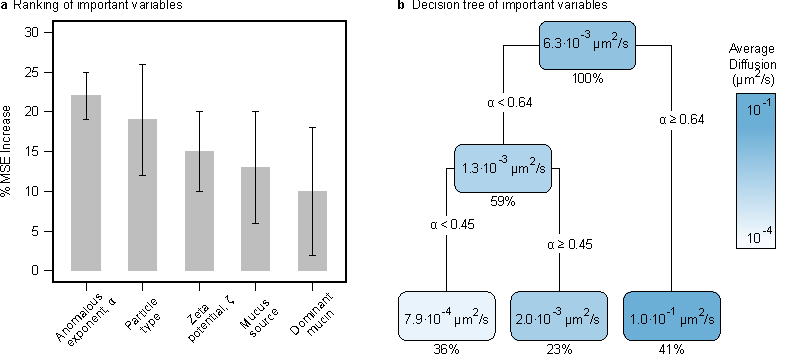
\includegraphics[width = 15 cm]{Figure_Random_forest_AL.pdf}
\caption{Selected variables impacting effective diffusion. $\textbf{a}$, Average percentage increase of mean-square error ($\%$ MSE) for the selected variables. The error bars correspond to the standard deviation. $\textbf{b}$, Decision tree for the most important variables. Each node contains the predicted average $D_{eff}$ and percentage of data predicted. The gradient display diffusion values from $\sim 10^{-4}$ $\upmu$m$^2$/s (white) to $\sim 10^{-1}$ $\upmu$m$^2$/s (blue).
}
\label{fig:randomforest}
\end{figure}

\clearpage

\begin{figure}
\centering
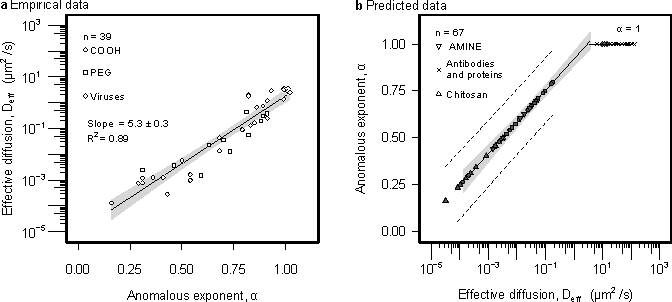
\includegraphics[width = 15 cm]{Figure_difvalp.pdf}
\caption{Effective diffusion and anomalous exponent analysis. $\textbf{a}$, effective diffusion was plotted as a function of the anomalous exponent. The solid line represents the regression model. The grey area represents the 95$\%$ confidence interval. Statistically significant slope and $R^2$ of linear regression are displayed. $\textbf{b}$, the anomalous exponent was predicted based on the model found empirically in $\textbf{a}$. The solid line designates the predicted linear model. The grey area represents the 95$\%$ confidence interval of the predicted linear model. The dashed line represents a 95$\%$ prediction interval \textbf{a-b}, distinguished particle types are represented in the legend of both panels.
}
\label{fig:difvalph}
\end{figure}  

\clearpage

\begin{figure}
\centering
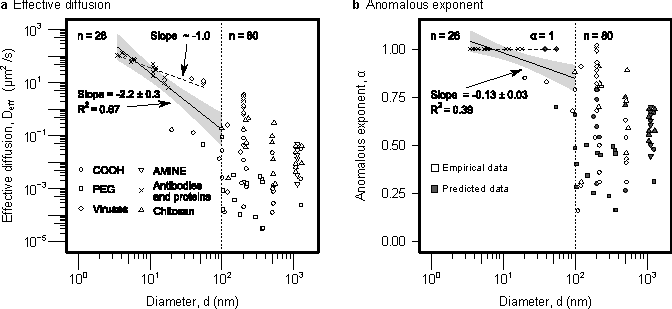
\includegraphics[width = 15 cm]{Figure_Size.pdf}
\caption{Particle size analysis.
\textbf{a}, The effective diffusion was plotted against particle size, d. The different symbols correspond to different particles types as indicated in the legend. The solid line indicates the linear regression for $d< 100$ nm particles using log-log data (n = 26), and it displays the slope and coefficient of determination, $R^2$. The grey area represents the 95$\%$ confidence interval. The group of particles with $d>100$ nm (n=80) did not display a statistically significant relationship and no solid line is included. The dashed line corresponds to the linear regression of the subset of particles (n = 21) displaying regular diffusion, $\alpha = 1$, in Fig. \ref{fig:difvalph}\textbf{b}, using the log-log data. The slope was appoximately one as expected ($slope = -1.0 \pm 0.1$, p-value = $1.4\cdot 10^{-7}$, $R^2=0.77$).
\textbf{b}, The anomalous exponent was plotted as a function of particle size. The symbols and lines are analogous to panel \textbf{a}. As in panel \textbf{a}, the solid line is the regression for the particles with  $d< 100$ (n = 26), while the dashed line represents the subset (n = 21) predicted to display regular diffusion, $\alpha = 1$. Empty symbols anomalous exponents obtained empirically. The solid symbols correspond to the predicted anomalous exponents for the subset of data that did not include empirical values. The predictions were obtained using the model derived from Figure \ref{fig:difvalph}\textbf{b}.
} 
\label{fig:SizeDiff}
\end{figure}

\clearpage

\begin{figure}
\centering
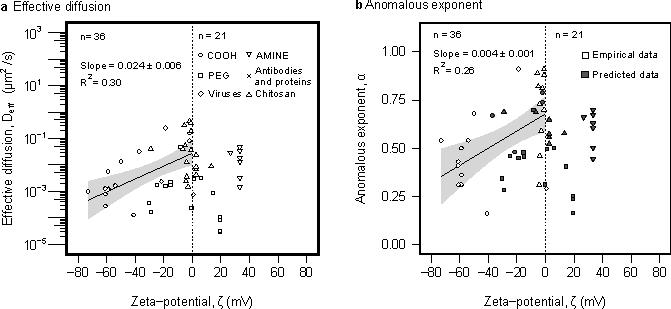
\includegraphics[width = 15 cm]{Figure_Charge.pdf}
\caption{Electrostatic analysis. \textbf{a} The effective diffusion was plotted against zeta potential. \textbf{b} The anomalous exponent was plotted as a function of zeta potential.  \textbf{a-b} The distinction between empirical and predicted data as well as particle types are represented in the legend. The dotted line indicates $\zeta = 0$.  The solid lines correspond to statistically significant linear regressions. The grey areas represent 95$\%$ confidence intervals of the linear regression. The slopes and $R^2$ of each linear regression are also displayed in the panels. 
}
\label{fig:ChargeDif}
\end{figure}  

\clearpage
%\end{linenumbers}
\end{document}
%
% ****** End of file apstemplate.tex ******

